\documentclass[11pt,a4paper,twoside,titlepage]{scrbook}
\usepackage[utf8]{inputenc}
\usepackage[pdfborder={0 0 0}]{hyperref}
\usepackage{amsmath}
\usepackage{amsfonts}
\usepackage{amssymb}
\usepackage{graphicx}
\usepackage{geometry}
\usepackage{tikz}
\usepackage{amsthm}
\usepackage{algorithmic}
\usepackage{algorithm}
\usepackage{float}
\usepackage{cleveref}
\usepackage{microtype}
\usepackage[ngerman]{babel}
\usepackage{complexity}
\usepackage{subcaption}


\usepackage{todonotes}
% \newcommand{\michael}[1]{\todo[inline]{MP: #1}}
% \newcommand{\fabian}[1]{\todo[inline,color=blue!20]{FA: #1}}
% \newcommand{\phillip}[1]{\todo[inline,color=yellow!20]{PK: #1}}
% \newcommand{\elisa}[1]{\todo[inline,color=red!20]{ES: #1}}
% \newcommand{\claudia}[1]{\todo[inline,color=red!20]{CA: #1}}


% allows you to skip the `figures/` part of paths in your \includegraphics
\graphicspath{{./figures/}}%

\theoremstyle{plain}%
\newtheorem{theorem}{Theorem}[chapter]
\newtheorem{lemma}[theorem]{Lemma}
\newtheorem{corollary}[theorem]{Corollary}

\newtheorem{proposition}[theorem]{Proposition}%

\theoremstyle{remark}%
\newtheorem{example}[theorem]{Example}%
\newtheorem{remark}[theorem]{Remark}%
\newtheorem{observation}[theorem]{Observation}%
\newtheorem{claim}[theorem]{Claim}%

\theoremstyle{definition}%
\newtheorem{definition}{Definition}[chapter]%

\crefname{figure}{Abbildung}{Abbildungen}
\crefname{chapter}{Kapitel}{Kapitel}
\crefname{definition}{Definition}{Definitionen}
\crefname{theorem}{Theorem}{Theoreme}
\crefname{lemma}{Lemma}{Lemmata}
\crefname{claim}{Behauptung}{Behauptungen}
\crefname{observation}{Beobachtung}{Beobachtungen}
\crefname{corollary}{Korollar}{Korollare}
\crefname{section}{Abschnitt}{Abschnitte}
\crefname{equation}{Formel}{Formeln}
\crefname{algorithm}{Algorithmus}{Algorithmen}
\crefname{table}{Tabelle}{Tabellen}


\DeclareMathOperator{\degree}{deg}
\DeclareMathOperator{\degrees}{deg^*}
\DeclareMathOperator{\flip}{flip}
\DeclareMathOperator{\flipDiag}{flip^*}
\DeclareMathOperator{\intersection}{I}
% \DeclareMathOperator{\convexhull}{CH^*}

\newcommand{\bigO}[1]{\mathcal{O}\left(#1\right)}
\newcommand{\myhspace}{\hspace{2cm}}

\begin{document}
\overfullrule=40pt
	\frontmatter

	%----- TITLE PAGE -----

	\begin{titlepage}
		%\noindent\makebox[\linewidth]{\rule{\paperwidth}{0.4pt}}

		\begin{tikzpicture}[remember picture, overlay]
		\node [anchor=north east, inner sep=0pt]  at (17.9,2)%(current page.north east)
			{
\includegraphics[height=3.5cm]{tu-bs_logo}};
		\end{tikzpicture}

		\centering
		\vspace{4cm}
		{\scshape\huge Bachelorarbeit\par}
		\vspace{1.5cm}
		{\Huge\bfseries Algorithmische Methoden zu gradbeschränkten Triangulierungen\par}
		\vspace{2cm}
		{\huge Fabian Alich\par}
		{\Large5310894\par}
		{\Large Informatik \par}

		\vfill\vfill
		Institut für Betriebssysteme und Rechnerverbund \\
        Abteilung Algorithmik\

		\vfill

		\textbf{Erstprüfer}\par
		Prof. Dr. Sándor Fekete \\ 
        Institut für Betriebssysteme und Rechnerverbund \\
        Abteilung Algorithmik\par
		\vfill

		\textbf{Zweitprüfer}\par
		Prof. Dr. rer. nat. Roland Meyer\\
        Institut für Theoretische Informatik\par
		\vfill
        
		\textbf{Betreuer}\par
		Dr. Phillip Keldenich\par
		Michael Perk\par
		\vfill
%\begin{description}
%	\item[Supervisor]
%	\item[First Reviewer]
%	\item[Second Reviewer]
%\end{description}


		% Bottom of the page
		{\large \today\par}
	\end{titlepage}

	\cleardoublepage

	% statement of originality
	\thispagestyle{plain} % no header
	\vspace*{7cm}
	\centerline{\bfseries Eigenständigkeitserklärung}
	\vspace*{1em}
	\noindent
	Hiermit versichere ich, dass ich die vorliegende Abschlussarbeit
selbstständig und ohne unzulässige fremde Hilfe erbracht habe. Ich habe
keine anderen als die angegebenen Quellen und Hilfsmittel benutzt. Die
wörtliche oder sinngemäße Übernahme von Abschnitten aus Texten
Dritter sowie aus eigenen vorangegangenen Veröffentlichungen habe ich
kenntlich gemacht.
\\ \\Ferner versichere ich, dass es sich hier um eine Originalarbeit handelt,
die noch nicht in einer anderen Prüfung vorgelegen hat.

	\par
	\bigskip\noindent Braunschweig, \today \par
	\vspace*{10mm}
	\hfill\hrulefill
	\cleardoublepage


	\chapter*{Aufgabenstellung}
	Eine Triangulierung einer Punktmenge ist die Zerlegung ihrer konvexen Hülle in nicht überlappende Dreiecke. Triangulierungen spielen eine zentrale Rolle in der algorithmischen Geometrie und finden vielfältige Anwendungen, etwa in der Computergrafik und geografischen Informationssystemen (GIS). Im Rahmen seiner Bachelorarbeit soll Herr Alich das neuartige kombinatorische Optimierungsproblem Degree-Constrained Triangulations (DCT) untersuchen. Bei diesem Problem geht es darum, für eine gegebene Punktmenge eine Triangulierung zu finden, bei der – zusätzlich zu den klassischen Anforderungen – die Knotengrade (also die Anzahl der angrenzenden Dreiecke bzw. Kanten pro Punkt) gewissen Beschränkungen unterliegen. Ziel der Arbeit ist es, geeignete Verfahren zur Lösung dieses Problems zu entwickeln, zu implementieren und zu evaluieren. Dabei können neben exakten Verfahren (z.B. auf Basis von Integer Programming, Constraint Programming oder Branch-and-Bound) auch heuristische Ansätze (z.B. Greedy- oder Metaheuristiken) betrachtet werden. Von besonderem Interesse sind außerdem Methoden zur Fixierung oder zum Ausschluss bestimmter Kanten, um die Lösungsräume gezielt einzuschränken sowie die Generierung von leichten und schweren Instanzen für das Problem.
    
    \par
	\bigskip\noindent Braunschweig, \today \par
	\vspace*{10mm}
	\hfill\hrulefill


	%---------------------
	\chapter*{Abstract}
This thesis examines the problem of degree constrained triangulations (DCT) where each vertex in a triangulation must have a given degree. 
Several exact and heuristic approaches were developed and implemented. 
These include edge based and triangle based encodings. 
In addition, strategies for fixing and excluding edges and systematic methods for generating instances for feasible and infeasible cases were introduced.

The experimental evaluation presents a comparison of different solvers such as PySAT, CaDiCaL, OR-Tools and Gurobi as well as various modeling techniques with respect to runtime and success rate. 
The results show that OR-Tools achieves the best results overall. 
All methods are only able to solve instances with a relatively small number of vertices. 
Optimization based formulations provide approximate solutions in infeasible or more complex cases.

The thesis shows that degree constrained triangulations can be effectively modeled and solved for small input sizes.
OR-Tools proves to be the most effective solver. 
The results provide a foundation for further research on scaling to larger instances and developing improved heuristics.

\fabian{ Ka wie ich das hier formatieren soll.}
\section{Deutsch}
Diese Arbeit behandelt das Problem der gradbeschränkten Triangulationen (Degree Constrained Triangulations, DCT), bei denen jedem Knoten einer Triangulation ein vorgegebener Grad zugeordnet wird. 
Hierfür wurden exakte und heuristische Lösungsansätze entwickelt und implementiert.
Dazu zählen kantenbasierte und dreiecksbasierte Kodierungen. 
Zusätzlich wurden Strategien zum Fixieren und Ausschließen von Kanten sowie systematische Verfahren zur Instanzgenerierung für lösbare und unlösbare Fälle entworfen.

Die experimentelle Untersuchung umfasst einen Vergleich verschiedener Solver wie PySAT, CaDiCaL, OR-Tools und Gurobi sowie unterschiedlicher Modellierungstechniken im Hinblick auf Laufzeit und Erfolgsquote. 
Die Ergebnisse zeigen, dass OR-Tools insgesamt die besten Resultate liefert. 
Alle Ansätze können jedoch nur Instanzen mit einer geringen Anzahl an Knoten lösen. 
Optimierungsbasierte Formulierungen liefern in unlösbaren oder komplexeren Fällen approximative Lösungen.

Die Arbeit zeigt, dass gradbeschränkte Triangulationen für kleine Eingabegrößen effizient modelliert und gelöst werden können. 
OR-Tools erweist sich dabei als leistungsfähigster Ansatz. 
Die Ergebnisse bilden eine Grundlage für weitere Forschung, insbesondere zur Skalierung auf größere Instanzen und zur Entwicklung verbesserter Heuristiken.

	\tableofcontents

	%% Remove listoffigures or listoftables if not needed!
	\listoffigures

	\listoftables

	\mainmatter
    % \fabian{Passen die ersten Titel so? Bin sehr unsicher wie ich die zusammenfassen soll.}

	%!TeX root=../thesis.tex
\chapter{Introduction}
\label{ch:introduction}%

You can write an introduction here!

\section{Results}
We proof that the \textsc{Traveling Salesmen Problem}(TSP) is NP-complete.
\begin{verbatim}
... that the \textsc{Traveling Salesmen Problem}(TSP) is ...
\end{verbatim}
You can use abbreviations for your problem names to avoid redundancy.
Try to use existing abbreviations from related work if possible.



\section{Related Work}
% What has been done in existing literature?
% This is needed to provide context of the area you are working in.

% You could for example cite~\cite{limper2013pop} with
% \begin{verbatim}
% ... example cite~\cite{limper2013pop} with
% \end{verbatim}
% The $\sim$ keeps two word in the same line but also separates with a space.
% Note that there is no space before the $\sim$.

% \section{Hints}
% For titles see \url{https://en.wikipedia.org/wiki/Title_case}.

% Leave an empty line to start a new paragraph.
% As a general rule: Never force line breaks.
% \begin{verbatim}
% Never use \\ or \newline
% \end{verbatim}

% You can add and refer to figures like \cref{fig:logo}.
% \begin{verbatim}
% ... figures like \cref{fig:logo}.
% \end{verbatim}
% The \verb|\cref{}| command automatically detects the reference type.

% \begin{figure}
% 	\centering
% 	
\includegraphics[]{tu-bs_logo}
% 	\caption[Short description]{Long description: Notice that the List of Figures has a shorter description than this text right here. Isn't this fascinating?}
% 	\label{fig:logo}
% \end{figure}

% Generally, we prefer a graph $G$ is \emph{complete} over \textbf{complete} if \ldots
% \begin{verbatim}
% ... graph $G$ is \emph{complete} over \textbf{complete} if \ldots.
% \end{verbatim}

Das ist meine Übersicht zur Related work

\subsection{Delaunay Triangulations}
Als Grundlage für den Algorithms können Delaunay Triangulation betrachtet werden.
Diese Liefern eine Triangulation welche möglichst Gleichschenklige Dreiecke nutzt.
In dem Buch von de Berg et.al.~\cite{Delaunay_Triangulation} wird diese Variante der Triangulation genauer betrachtet.
In diesem Fall wird mit den Delaunay Triangulation das Problem gelöst, das höhendaten in einem zwei Dimensionalen Raum dargestellt werden.

Triangulation eignen sich aufgrund ihres Aufbaues gut um Höhendaten im zwei Dimensionalen Raum darzustellen (siehe Bild ~\ref{fig:terrain}).
Hier kann genutzt werden das Dreiecke verschiedene Innenwinkel und Kantenlängen haben können.
\begin{figure}[tb]
	\caption{\emph{A perspective view of a terrain} aus ~\cite[p.~183]{Delaunay_Triangulation}}
	\centering
	\label{fig:terrain}
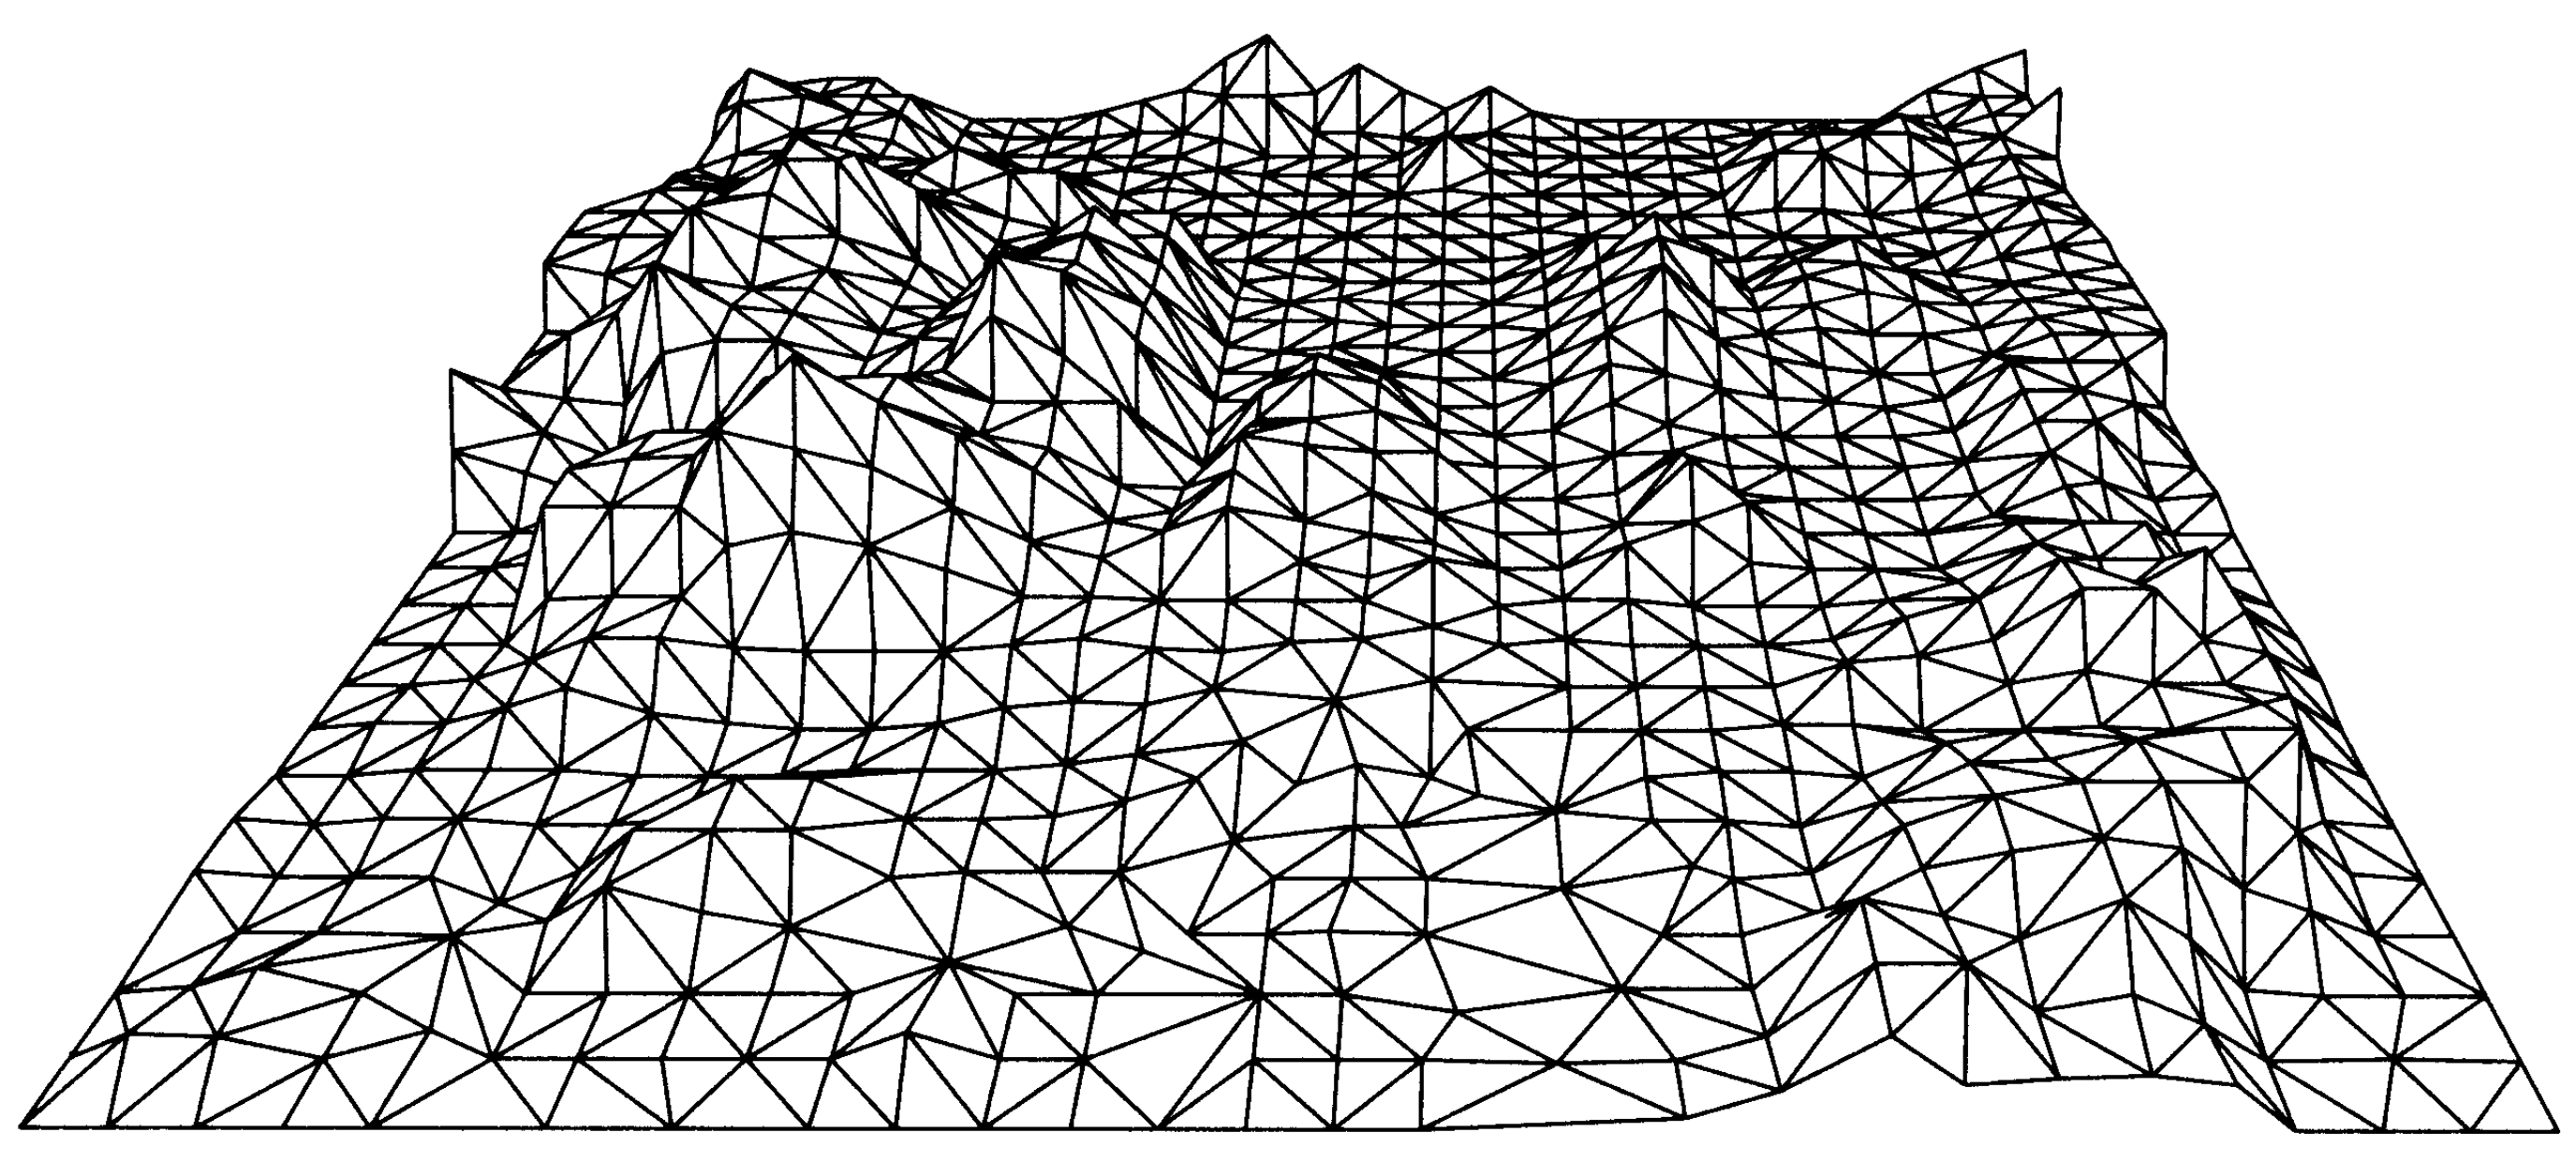
\includegraphics[scale=0.2]{Delauney_Tarrain.png}
\end{figure}
Das Grundproblem ist hier das die höhendaten nur an bestimmten Punkten bekannt sind und somit die Restlichen Höhendaten erraten werden müssen.

\begin{itemize}
	\item für die darstellung Höhen raten
	\item Gleichschenklich sieht am besten aus
	\item ziel minimalen Winkel maximieren
	\item Formel für Kanten und Dreiecke bekommen
	\item drei Algos
\end{itemize}

\subsection{Flips in Triangulations}
Flips sind Möglichkeiten, um Kanten in einer Triangulation auszutauschen.
Da Triangulationen für die gleiche Knotenmenge, wie in~\cite{Delaunay_Triangulation} erwähnt, stets die gleiche Anzahl an Kanten besitzen, können keine Kanten hinzugefügt oder entfernt werden, um den Grad einer Triangulation zu verändern.
Daraus folgt, dass für jede entfernte Kante eine andere Kante eingefügt werden muss.
Eine besondere Art dieser Umstrukturierung von Kanten sind sogenannte Flips.
Hurtado et al.~\cite{Flipping_edges_in_triangulations} zeigten, dass jede Triangulation mindestens
\[\frac{n-4}{2}\]
flipbare Kanten besitzt, wobei \( n \) die Anzahl der Knoten bezeichnet.
Laut dem Paper \emph{Flips in planar graphs}~\cite{Flips_in_planar_graphs} lässt sich jede mögliche Triangulation in jede beliebige andere Triangulation überführen, indem die notwendigen Flips durchgeführt werden.
Daraus folgt, dass, wenn eine \emph{degree-constrained triangulation} möglich ist, diese mit den nötigen Flips konstruiert werden kann.

Eine weitere Art von Flips sind sogenannte \( k \)-Flips.
Diese stellen eine zusätzliche Möglichkeit dar, Kanten innerhalb einer Triangulation zu verschieben.
Dabei werden \( k \) Kanten entfernt und durch \( k \) neue Kanten ersetzt.
Normale Flips entsprechen somit \( 1 \)-Flips.
Der Vorteil von \( k \)-Flips liegt darin, dass mit einem Schritt größere strukturelle Veränderungen möglich sind.

\textbf{Absatz für Flips mit Binärbäumen hinzufügen, falls verwendet.}

\begin{figure}[ht]
  \centering
  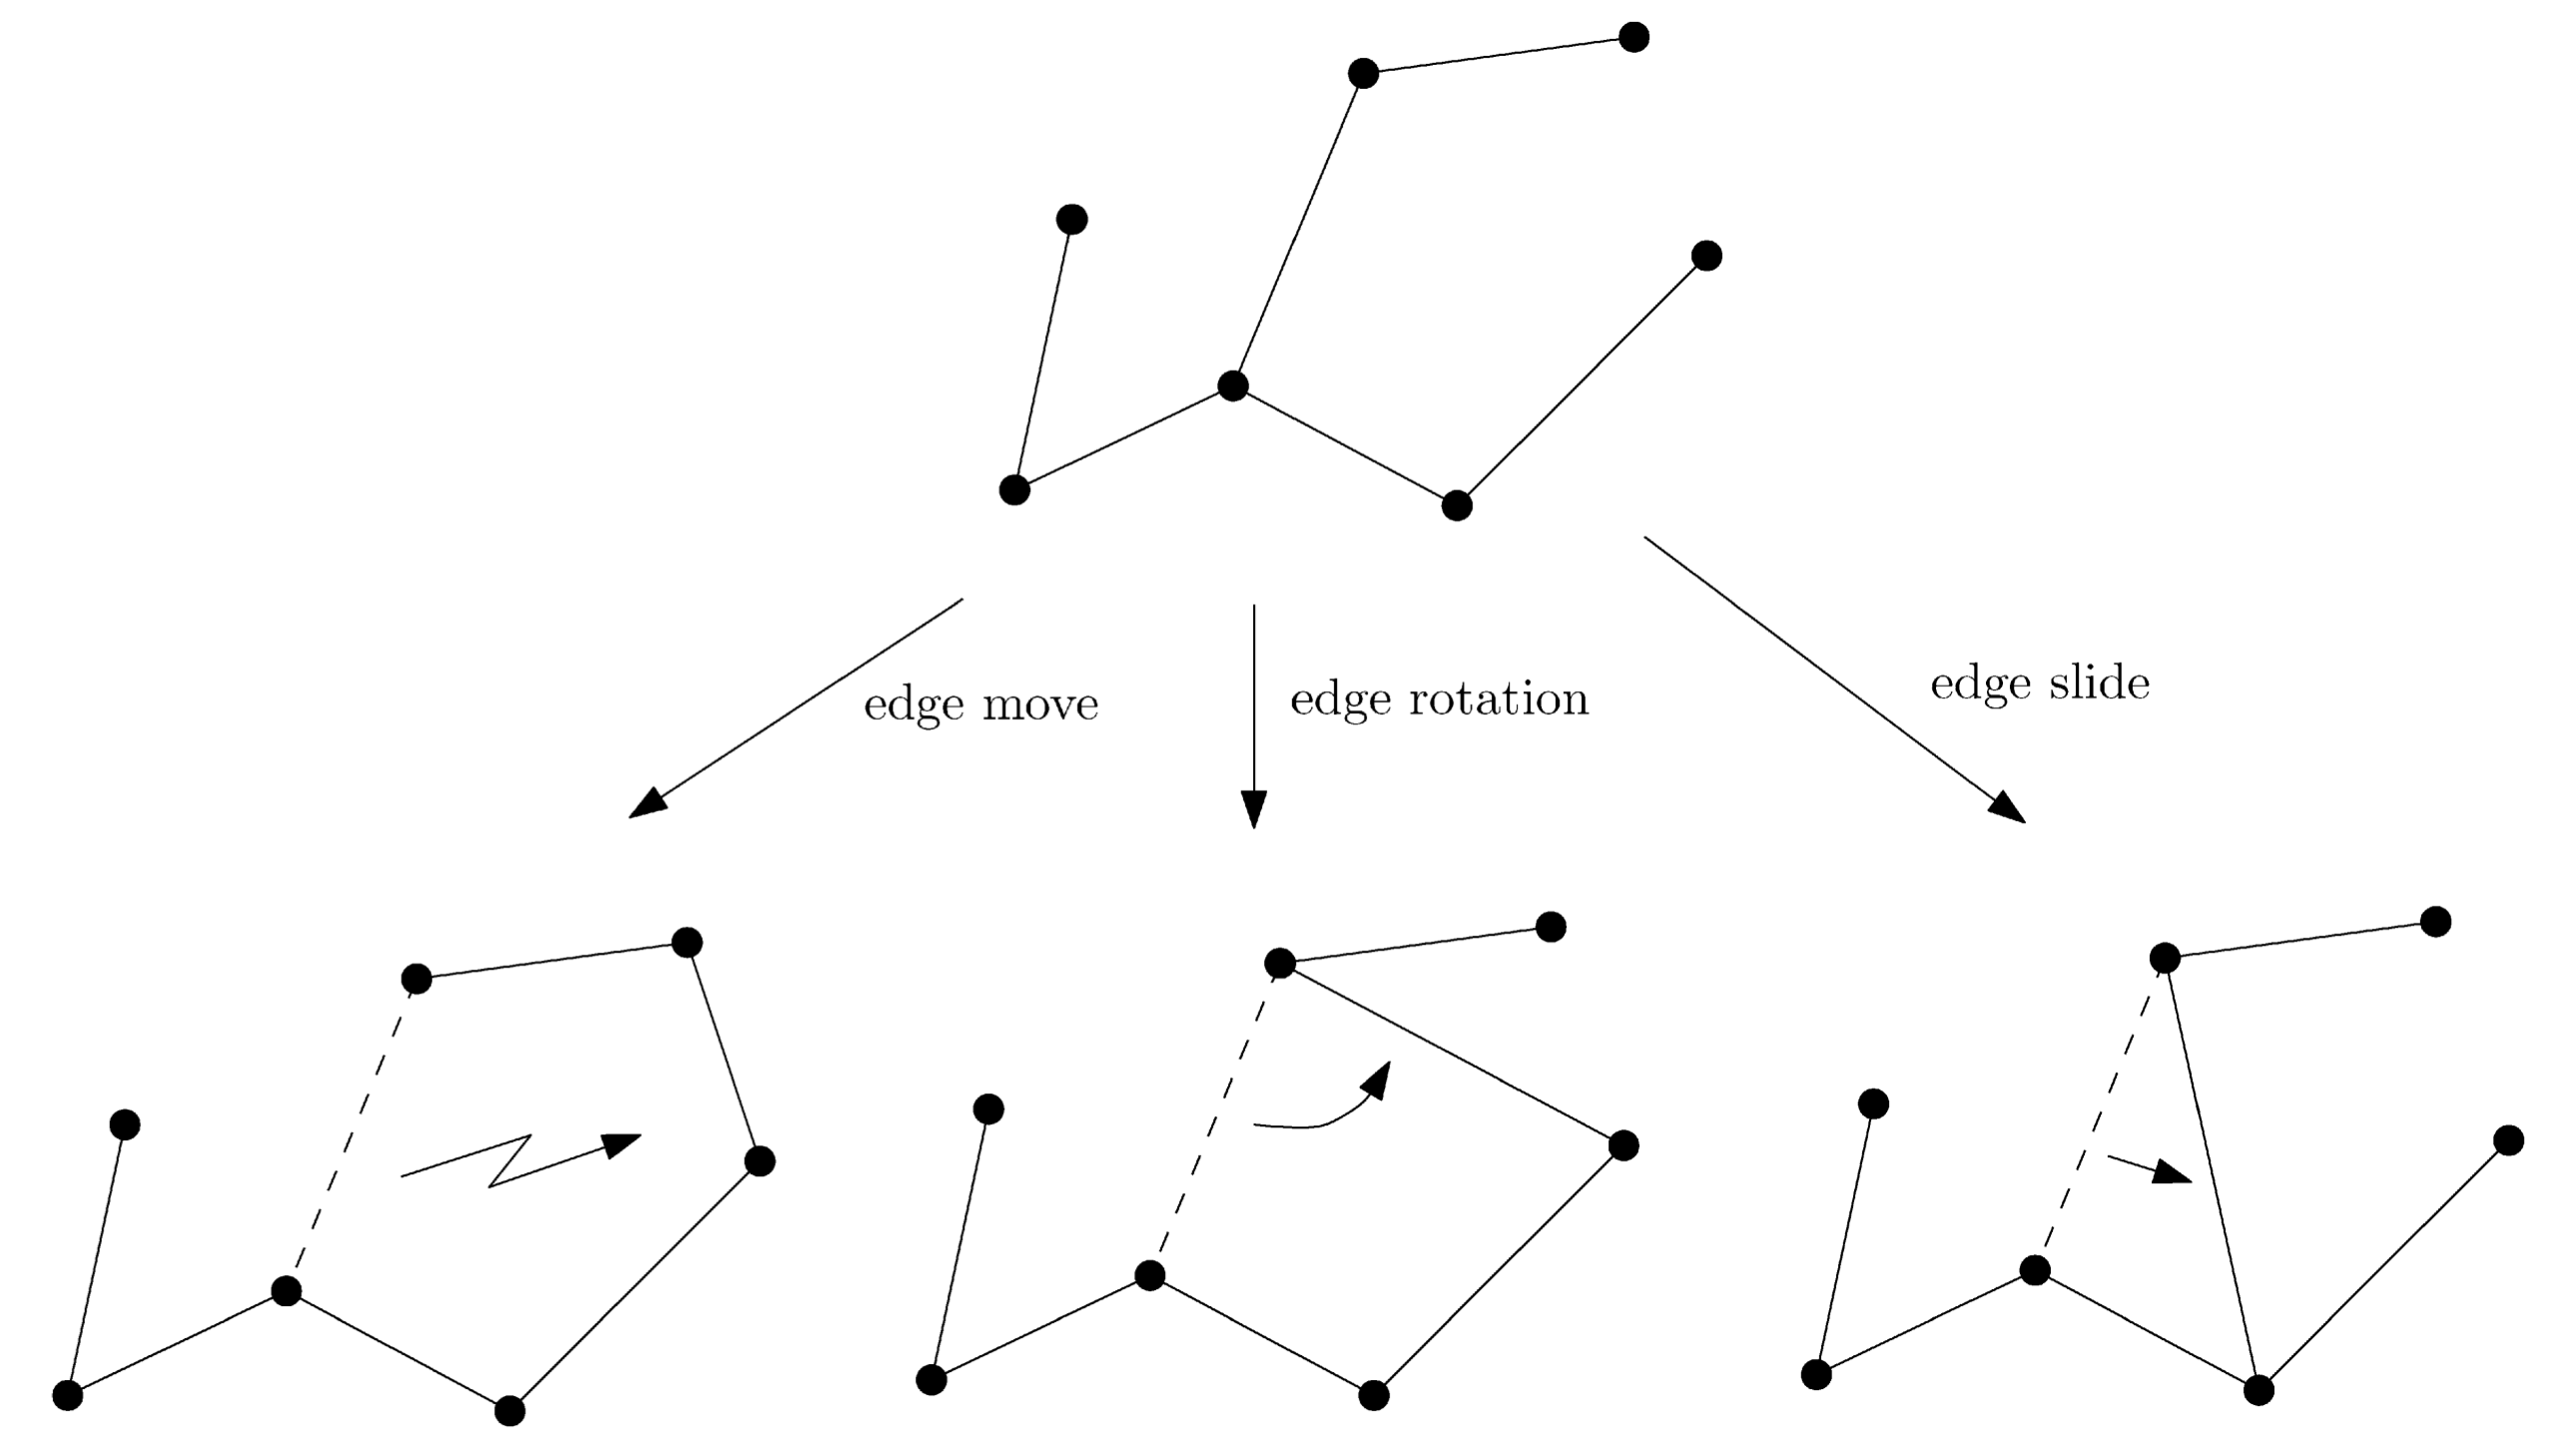
\includegraphics[width=\linewidth]{drei_flips.png}
  \caption{\emph{Examples of edge move, edge rotation, and edge slide} aus~\cite[p.~70]{Flips_in_planar_graphs}}
  \label{fig:drei_flips}
\end{figure}

Drei beispielhafte Flips sind in Abbildung~\ref{fig:drei_flips} dargestellt.
Zum einen der \emph{edge move}, hierbei handelt es sich um das einfache Entfernen und anschließende Einfügen einer Kante.
Etwas stärker eingeschränkt ist die \emph{edge rotation}, bei der ein Endpunkt der Kante unverändert bleibt.
Die Rotation erfolgt also nur um einen Knoten.
Die dritte Variante, der \emph{edge slide}, schränkt die \emph{edge rotation} weiter ein.
Hier darf der veränderte Knoten nur ein Nachbar des ursprünglichen Knotens sein.

\subsection{degree constrained minimum spanning tree}
das sind viele infos

zum beispiel das brand and bound genutzt wird



\section{Overview}
If needed, write down where to find everything.

	\chapter{Preliminaries}

\begin{definition}[Überschneidung]
	Zwei Kanten gelten als Schneidet wenn sie sich in der Ebene kreuzen.
	Im Folgendem werden mit der Funktoin \(I: ( \mathbb{Z}^2, \mathbb{Z}^2) \longrightarrow \{\mathbb{Z}^2\}\) alle Kanten angegeben, die die übergebene Kante schneiden.
\end{definition}
\begin{definition}[Planarer Graph]
	Ein Planarer Graph ist ein Graph ohne überschneiden Kanten.
	Das bedeutet man kann alle Punkte und Kanten darstellen ohne das sich diese überschneiden.
\end{definition}
\begin{definition}[Triangulation]
	Eine Triangulation einer Punktemenge \(P \in \mathbb{Z}^2\) ist ein Maximaler Planarer Graph.
	Das bedeutet man kann keine weiteren Kanten hinzufügen ohne das sich diese Schneiden.
\end{definition}
\begin{theorem}
	TODOGehört Sowas hier hin? Soll ich sowas nennen


	Alle Flächen außer der Äußeren Fläche einer Triangulation bestehen aus Dreiecken.
	Der Beweis wird von Mark Berg et.al. geliefert\cite[p.~185]{Delaunay_Triangulation}.
\end{theorem}
\begin{definition}[Grad]
	Der Grad gibt die Anzahl der anliegenden Kanten an einem Knoten an.
	Im folgenden wird er durch die Funktion \(\degree: \mathbb{Z}^2 \longrightarrow \mathbb{Z}\) angegeben.
\end{definition}
\begin{definition}[Gradbeschränkte Triangulation]
	Die Gradbeschränkte Triangulation hat die gleichen Vorraussetzungen wie eine Triangulation.
	Zusätzlich gibt es noch eine Funktion \(\degrees: \mathbb{Z}^2 \longrightarrow \mathbb{Z}\).
	Diese gibt den Grad an welcher ein Knoten haben muss.
\end{definition}
\begin{definition}[Flipp]
	Eine Operation bei der eine Kante entfernt und eine andere Hinzugefügt wird.
	Hierbei dürfen nach der Operation die Triangulations Eigenschaften nicht verletzt sein.
	Ein Flip wird durch die Funktion \(\flip:(\mathbb{Z}^2,\mathbb{Z}^2) \longrightarrow (\mathbb{Z}^2,\mathbb{Z}^2)\) definiert.

\end{definition}
\begin{definition}[Diagonale Flipp]
	Ein Diagonaler Flipp hat die gleichen Eigenschaft wie ein Flipp.
	Zusätzlich wird für die Kante \((b,c)\) die leeren Dreicke \(\triangle abc \) und  \(\triangle bcd \) gesucht und \((a,d)\) zurückgeben.
	Er wird durch die Funktion \(\flipDio:(\mathbb{Z}^2,\mathbb{Z}^2) \longrightarrow (\mathbb{Z}^2,\mathbb{Z}^2) definiert\).
\end{definition}

	\chapter{Content}

\section{Instanzen Generation}
\subsection{Ja - Instanzen}
Bei den Ja-Instanzen handelt es sich um Punktmengen bei denen die \(\degrees\) Funktion Grade liefert welche eine Gradbeschränkte Triangulation ermöglichen. 
Hierbei ist nicht bekannt wie viele mögliche Lösungen es gibt nur das es mindestens eine gibt.
Der Generelle Ablauf fängt mit einer zufälligen Punktmenge an.
Hierbei wird nur die Anzahl der Punkte vorgegeben.
Danach wird mit einem klassischen Verfahren eine Triangulation erstellt.
Von dieser werden dann die Grade und die Knoten gespeichert.
\subsubsection{Delaunay mit zufälligen Flips}
Das erste klassische Verfahren zur Grad bestimmung ist die Delaunay Triangulation in verbindung mit Flips.
Die Delaunay Triangulation wurde im Kapitel~\ref{sec:delaunay_triangulation} bereits vorgestellt.
Für die erstellung der Delaunay Triangulation wird die Bibliothek \texttt{scipy} genutzt.
Auf dieser Triangulation werden dann \(k\) mal die in~\cref{def:flip} Definierten Flips durchgeführt.
Für die durchführung eines Flips zufällig eine Kante \(e_0\) ausgewählt.
Für diese Kante werden zunächst alle Dreiecke gesucht die diese Kante enthalten.
Dies geschied in dem für die beiden Knoten \(x_{0.0}\) und \( x_{0.1}\) der Kante \(e_0\) alle ausgehende Kanten vergleichen werden.
Sollte zwei dieser Kanten den gleichen Knoten  \(v\) haben muss das Tripel (\(x_{0.0}, x_{0.1}, v\)) ein Dreieck sein welches die Kante \(e_0\) enthält.
Sollten am Ende mehr als zwei Dreicke gefunden werden, so müssen die beiden Dreicke ausgewählt werden welche leer sind. 
Hierbei kann es nur zwei lerrer Dreicke geben da es in einer Triangulation nicht zu überschneidungen kommen darf.
Von diesen beiden Dreicken (\(x_{0.0}, x_{0.1}, v_0\)) und (\(x_{0.0}, x_{0.1}, v_1\)) wird dann die Kante \(e_0\) durch die Kante bestehend aus \(v_0\) und \(v_1\) ersetzt.
\subsubsection{Random Kanten}
Bei der zweiten klassischen Triangulation werden zufällig Kanten hinzugefügt.
Hierbei werden zunächst alle möglichen Kanten zwischen den Punkten erstellt.
Bei diesem Schritt werden Kanten ausgeschlossen welche einen anderen Punkt schneiden.
Diese Kanten werden dann in einer zufälligen Reinfolge betrachet.
Bei der auswahl der finalen Kanten wird geprüft ob die Kante eine der zuvor ausgewählten Kanten schneidet.
Sollte dies nicht der Fall sein wird die Kante ausgewählt.
Dieses Verfahren ist maximal da wird alle möglichen Kanten betrachten.

\subsection{Nein - Instanzen}
\begin{itemize}
	\item Move Point liefert meistens nein Instanzen
	\item Zwei Sollgrade von zwei Punkten Tauschen
\end{itemize}
\section{Heuristiken}
\begin{itemize}
	\item eine Triangulation erstellen
	\item den sollGrad möglichst richtig
	\item Werden mit folgender Formel bewertet
\end{itemize}

\begin{align}
 \text{diff}_i &= \left| \degrees(i) - \degree(i) \right| \label{eq:difference} \\
e_i &= \left\{
\begin{array}{ll}
\frac{\degrees(i) - \text{diff}_i}{\degrees(i)} & \degrees(i) \geq \text{diff}_i \\
0 & \, \textrm{sonst} \\
\end{array}
\right. \label{eq:evaluation}\\
Q_T &= \sum_{i=0}^{n} \frac{e_i}{n} \label{eq:total_evaluation}
\end{align}

Die Formel liefert eine Evaluation (\(Q_T\)) für einen Triangulation(\(T\)) mit \(n\) Knoten.
Hierbei gibt \(\degrees(i)\) den gewünschten Grad an der stelle i an.
Dazu passend gibt \(\degree(i)\) den aktuellen Grad an.
In der Brechnung~\eqref{eq:difference} wird die Difference zwischen dem gewünschten und aktuellen Grad berechnet.
In~\eqref{eq:evaluation} wird diese Abweichung Prozentual bewertet.
Am Ende wird in~\eqref{eq:total_evaluation} ein Durchschnitt über alle Prozentualen Werte gebildet.

\subsection{Flips}
\begin{itemize}
	\item Diagonale Flips
	\item k mal Wiederholen
	\begin{itemize}
		\item Alle Knoten durchgehen
		\item wenn falscher Degree auswählen
		\item alle ausgehenden Kanten berechnen
		\item Kante Auswählen \cref{algo:choose_edge}
		\item Flipe Kante wie oben
		\item wenn Gradbeschränkte Triangulation erfolgreich abbrechen
	\end{itemize}
\end{itemize}
\begin{algorithm}[H]
	\caption{CHOOSE EDGE(\(v\))}
	\label{algo:choose_edge}
	\begin{algorithmic}[1]
		\STATE \(E \gets \{ e \mid e \text{ ist ausgehende Kante von } v \}\)
		\WHILE{\(E \neq \emptyset\)}
			\STATE \(e \gets \) zufälliges Element aus \(E\)
			\STATE \(E \gets E \setminus \{e\}\)
			\STATE \(u \gets \text{Knoten von } e~\AND~v \neq u\)
			\IF{\(\degree(u) \neq \degrees(u)\)}
				\RETURN e
			\ELSIF{zu 20 \%}
				\RETURN e
			\ENDIF
		\ENDWHILE
		\RETURN e
	\end{algorithmic}
\end{algorithm}
\subsection{OrTools mit Zielfunktion}
\label{sec:ortools_heu}
TODO infos über OrTools rausuchen
\begin{itemize}
	\item Solver von Google
	\item Solver mit intersection Konstriend und Zielfunktion maximiere~\eqref{eq:evaluation}
	\item erste Konstriend Kanten auf richtige Anzahl
\end{itemize}
Zunächst sei \(E\) die Menge aller Kanten und \(E_P\) die Menge aller möglicher Kanten. Also Kanten die keine Punkte schneiden.
Für jede Kante \(e \in E\) wird eine Bool Variable \(x_e\) erstellt.
Diese Variable ist wahr wenn die Kante \(e\) in der Triangulation enthalten ist.
Für den Überschneidungs Konstriend werden folgende Klauseln dem OrTools Modeln hinzugefügt.
\[
\neg x_{e_1} \lor \neg x_{e_2} \hspace{3cm} \forall e_1, e_2 \in E_P: e_2 \in \intersection(e_1) 
\]
\begin{itemize}
	\item Zielfunktion ist maximiere \(Q_T\) aus~\eqref{eq:evaluation}
	\item Teiler rausgenommen da für max nicht relevant
	\item für die Difference, Betrag und min muss eine Integer Hilfsvarible eingeführt werden.
\end{itemize}
\begin{itemize}
	\item Zweiter ansatz weniger Integer Variablen nutzen
	\item Degree - sollDegree und sollDegree - Degree größer als Hilfsvarible
	\item Summe maximieren
\end{itemize}

\section{Solver}
\begin{itemize}
	\item Exakte Ergebnise Liefern die Triangulation und Gradbeschränkung erfüllen
	\item alle Solver desten ob sum(degree) = 2* Kanten für Triangulation
\end{itemize}
\subsection{OrTools}
\begin{itemize}
	\item gleicher Solver jetzt mit Gradbeschränkung
	\item Kanten Variblen und Intersection Konstriend wie in~\cref{sec:ortools_heu}
	\item Zwei Grundansätze 
	\begin{itemize}
		\item Kanten Maximieren und dann nach Lösung abbrechen welche richtige Anzahl Kanten hat
		\item Kanten Anzahl festsetzen und ohne Zielfunktion lösen
	\end{itemize}	
	\item Ansatz für die Gradbeschränkung
	\item für jeden Knoten die summe der x für ausgehende Kanten varibalen gleich dem Sollgrad
\end{itemize}	
\subsection{SAT mit Kanten}
TODO Rausfinden wie SAT degree gemacht wird
\begin{itemize}
	\item Alle möglichen Kanten als Bool Variable wie OrTools
	\item Intersection Konstriend wie OrTools
	\item Degree sat mit eingebauter Funktion(Infos raussuchen)
	\begin{itemize}
		\item Hilfsveriablen ab max(len(all\_vars), höchste var in solver) + 1
	\end{itemize}
	\item das waren Grundlagen jetzt Verbesserungen
	\item Kanten Anzahl fest setzen
	\item Convexe Hülle festsetzen
	\item Intersection mit Algo Von Michael
	\item Satformel aus Paper von Michael, Fekete und Phillip Alle Edges
	\item Subset degree
	\begin{itemize}
		\item alle Knoten durchgehen
		\item alle Kombinationen der größe len(enges) - (degree -1) bilden
		\item als Klauseln hinzufügen
		\item Als Bild erklären
	\end{itemize}
	\item Bei degree nicht genau degree sondern nur mindestens degree
	\item muss reichen weil sonnst ein anderer Knoten nicht genügend Kanten bekommt
	\item exclude Edges
	\begin{itemize}
		\item alle Kanten betrachten welche die Punkt menge teilen
		\item testen ob anzahl kanten * 2 = sum(degree)
	\end{itemize}
\end{itemize}
\section{SAT mit Dreicken}
\begin{itemize}
	\item Alle möglichen Dreicke erstellen
	\item Spätere Verbesserung nur Leere Dreicke
	\item jedes Dreieck als Bool Variable
	\item Intersection Konstriend wie bei Kanten 
	\item Degree normaler Knoten degree = sum(Dreicke)
	\item Degree auf Convexe Hülle degree - 1 = sum (Dreicke)
\end{itemize}
\section{Theoretische Mehrere Lösungen}
TODO Wo soll das hin
\begin{itemize}
	\item 3 und 4 Knoten ist Gradbeschränkte Triangulation immer eindeutig
	\item ab 8 bis unentlich gibt es mehrere Lösungen
	\item instaze zeigen und erklären wie mehr Punkt hinzufügen
\end{itemize}
	\chapter{Auswertung}
\section{Versuchsumgebung}
\begin{itemize}
	\item Implementation details (e.g., libraries, third-party programs, \dots)
	\item In which environment are you testing (e.g., system specifications)
	\item What are you testing? (e.g., runtime, space needed, fps, \dots)
	\item What are the results? Show fancy figures!
	\item What does the results mean? (e.g., give a little discussion on your results)
	\item \dots
\end{itemize}

\section{Grund Solver (Eval1)}

\subsection{Dreiecke}
\begin{figure}[tb]
    \centering
    
\includegraphics[width=1\linewidth]{figures/eval1/tri.pdf}
    \caption{Enter Caption}
\end{figure}

{%
  \catcode`\_=12 % Unterstrich als normales Zeichen
  \catcode`\#=12 % Rautenzeichen als normales Zeichen
    \obeylines
    \input{figures/eval1/tri.txt}
}
\subsection{Sat}
\begin{figure}[tb]
    \centering
    
\includegraphics[width=1\linewidth]{figures/eval1/sat.pdf}
    \caption{Enter Caption}
\end{figure}

{%
  \catcode`\_=12 % Unterstrich als normales Zeichen
  \catcode`\#=12 % Rautenzeichen als normales Zeichen
    \obeylines
    \input{figures/eval1/sat.txt}
}
\subsection{OrTools}
\begin{figure}[tb]
    \centering
    
\includegraphics[width=1\linewidth]{figures/eval1/ortools.pdf}
    \caption{Enter Caption}
\end{figure}

{%
  \catcode`\_=12 % Unterstrich als normales Zeichen
  \catcode`\#=12 % Rautenzeichen als normales Zeichen
    \obeylines
    \input{figures/eval1/ortools.txt}
}
\subsection{Gurobi}
\begin{figure}[tb]
    \centering
    
\includegraphics[width=1\linewidth]{figures/eval1/gurobi.pdf}
    \caption{Enter Caption}
\end{figure}

{%
  \catcode`\_=12 % Unterstrich als normales Zeichen
  \catcode`\#=12 % Rautenzeichen als normales Zeichen
    \obeylines
    \input{figures/eval1/gurobi.txt}
}
\subsection{Gesamt}
\begin{figure}[tb]
    \centering
    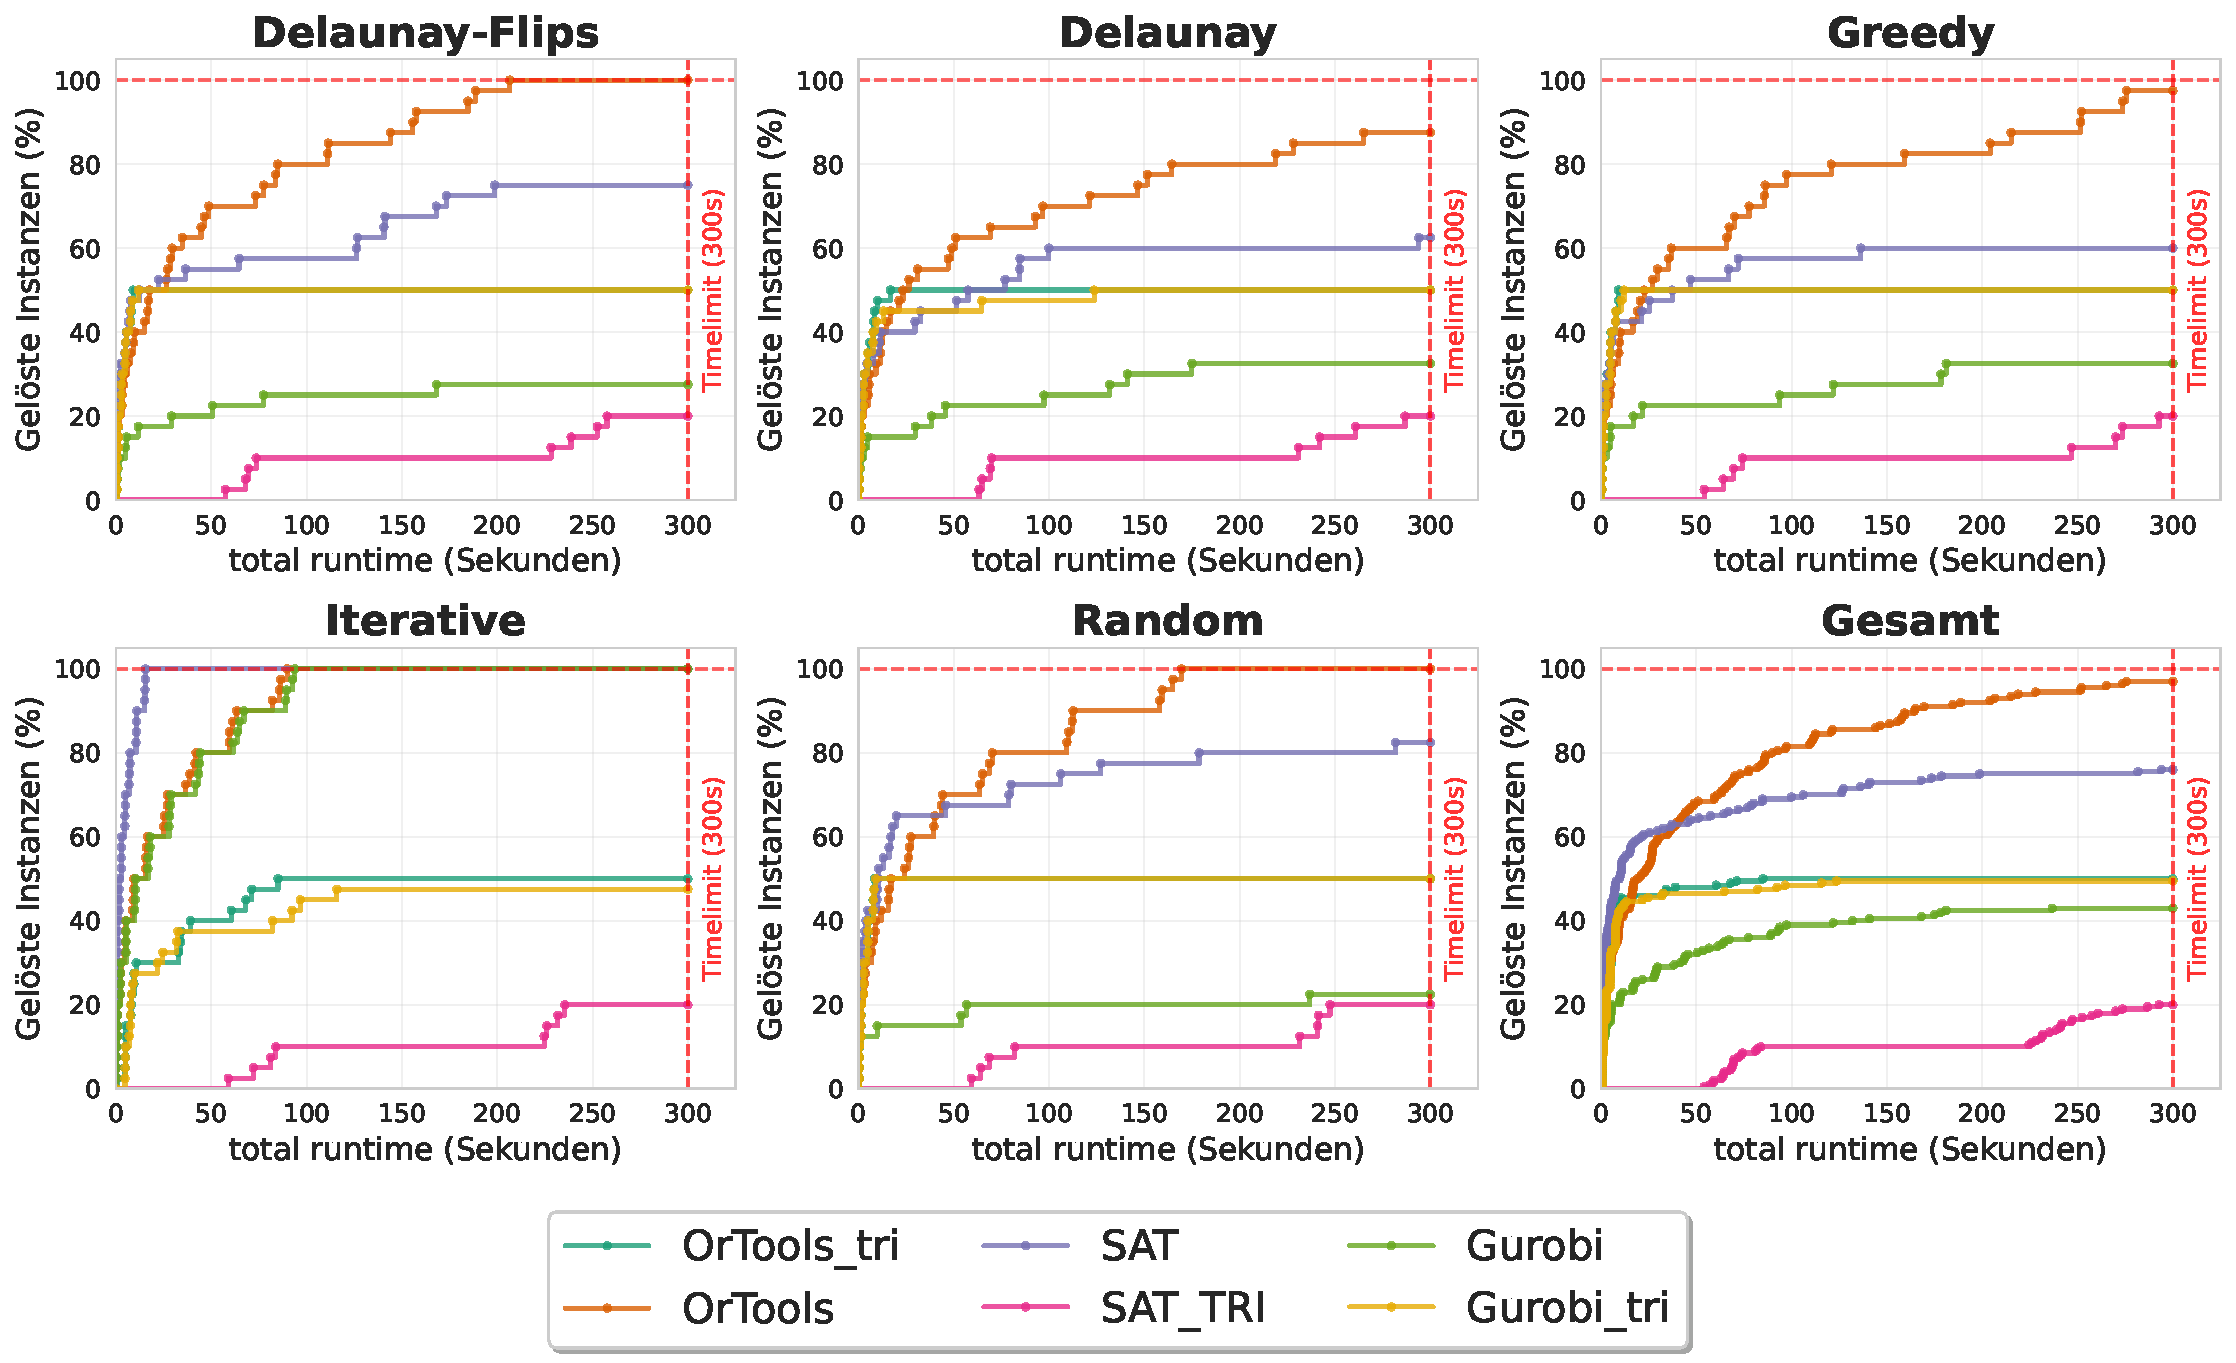
\includegraphics[width=1\linewidth]{figures/eval1/gesamt.pdf}
    \caption{Enter Caption}
\end{figure}

{%
  \catcode`\_=12 % Unterstrich als normales Zeichen
  \catcode`\#=12 % Rautenzeichen als normales Zeichen
    \obeylines
    \input{figures/eval1/gesamt.txt}
}




	\chapter{Fazit und Ausblick}
In dieser Arbeit wurde das neuartige Problem DCT untersucht. 
Dabei erfolgte die Betrachtung sowohl als Entscheidungsproblem als auch Optimierungsproblem. 
Für das Entscheidungsproblem wurden zwei Modellierungen entwickelt, eine kantenbasierte und eine dreiecksbasierte Formulierung. 
Darüber hinaus wurden fünf verschiedene Instanztypen konstruiert, um sowohl lösbare als auch unlösbare Fälle zu erzeugen.
Bei der kantenbasierten Modellierung zeigte sich, dass OR-Tools in Kombination mit der Fixierung der Hülle sowie ausgewählter möglicher Kanten und unter Einbezug der alternativen Kantenbeschränkung die besten Ergebnisse erzielte. 
Mit diesem Ansatz konnten Instanzen mit einer Knotenanzahl von bis zu 220 gelöst werden. 
Für jede getestete Instanzart konnten mindestens 170 Knoten erfolgreich gelöst werden. 

Auch bei der dreiecksbasierenden Modellierung lieferte OR-Tools die besten Resultate. 
Es konnte festgestellt werden, dass diese Modellierung für alle Instanztypen, unabhängig von ihrer vermeintlichen Schwierigkeit, vergleichbare Ergebnisse erzielte. 
Zusätzlich wurde mit dem CDCL-Ansatz eine theoretische Möglichkeit aufgezeigt, den Lösungsprozess weiter zu optimieren. 
Dennoch bleibt die Skalierbarkeit auf große Instanzen eine zentrale Herausforderung, da die vorgestellten Verfahren insbesondere für kleinere Knotenmengen praktikabel sind. 
Darüber hinaus zeigte sich, dass die Struktur der Instanzen, insbesondere die Verteilung der Kantenlängen und Knotengrade, bei der kantenbasierten Formulierung einen erheblichen Einfluss auf die Schwierigkeit der Instanz hat.

Ein vielversprechender Ausblick besteht darin, die vorgestellten Verfahren im Hinblick auf ihre Skalierbarkeit zu verbessern. 
Eine interessante Möglichkeit wäre, den Arbeitsspeicherverbrauch der Ansätze systematisch zu vergleichen, da dieser insbesondere bei großen Instanzen zu Problemen geführt hat. 
Ebenso könnte die dreiecksbasierte Modellierung genauer untersucht werden, um zu verstehen, weshalb alle Instanztypen als ähnlich schwierig erschienen. 
Genauso interessant wäre es zu untersuchen, warum bei der Kantenbedingung die Optimierungen bei OR-Tools in Kombination geholfen haben und bei PySAT und Gurobi nur einzeln.
Darüber hinaus bietet der \emph{Propagation}-Ansatz weiteres Potenzial, da hierbei die Eigenschaft genutzt werden könnte, dass Kanten isoliert in Teilinstanzen auftreten. 
So können diese Kanten genutzt werden, um mit zwei weiteren die Instanz zu halbieren.
Schließlich wäre es interessant, bei der Instanzgenerierung normalverteilte Triangulierungen zu berücksichtigen, um einheitlichere und realistischere Szenarien abzubilden.

Ein interessante Abwandlung des Problems wäre es, wenn in der Triangulierung Kanten vorgegeben sind, die immer genutzt werden müssen.
Dies wurde in~\cref{sec:kanten_vorab_berechnen} teilweise betrachtet, aber nicht als eigenes Problem.
Dieses Problem könnte man noch weiter abwandeln, indem man keine Knotenmengen, sondern Polygone mit und ohne Löcher nutzt.
Auch könnte man das in~\cref{sec:einleitung:min-degree} genannte \emph{Min-Degree Constrained Minimum Spanning Tree} abwandeln, sodass der Sollgrad exakt und nicht als Mindestgrad betrachtet wird.



	\bibliographystyle{plainurl}
	\bibliography{bibliography}
	% !TeX root = ../thesis.tex
\appendix

\chapter{SAT Degree Auswertung}
\begin{figure}[htb]
    \centering
    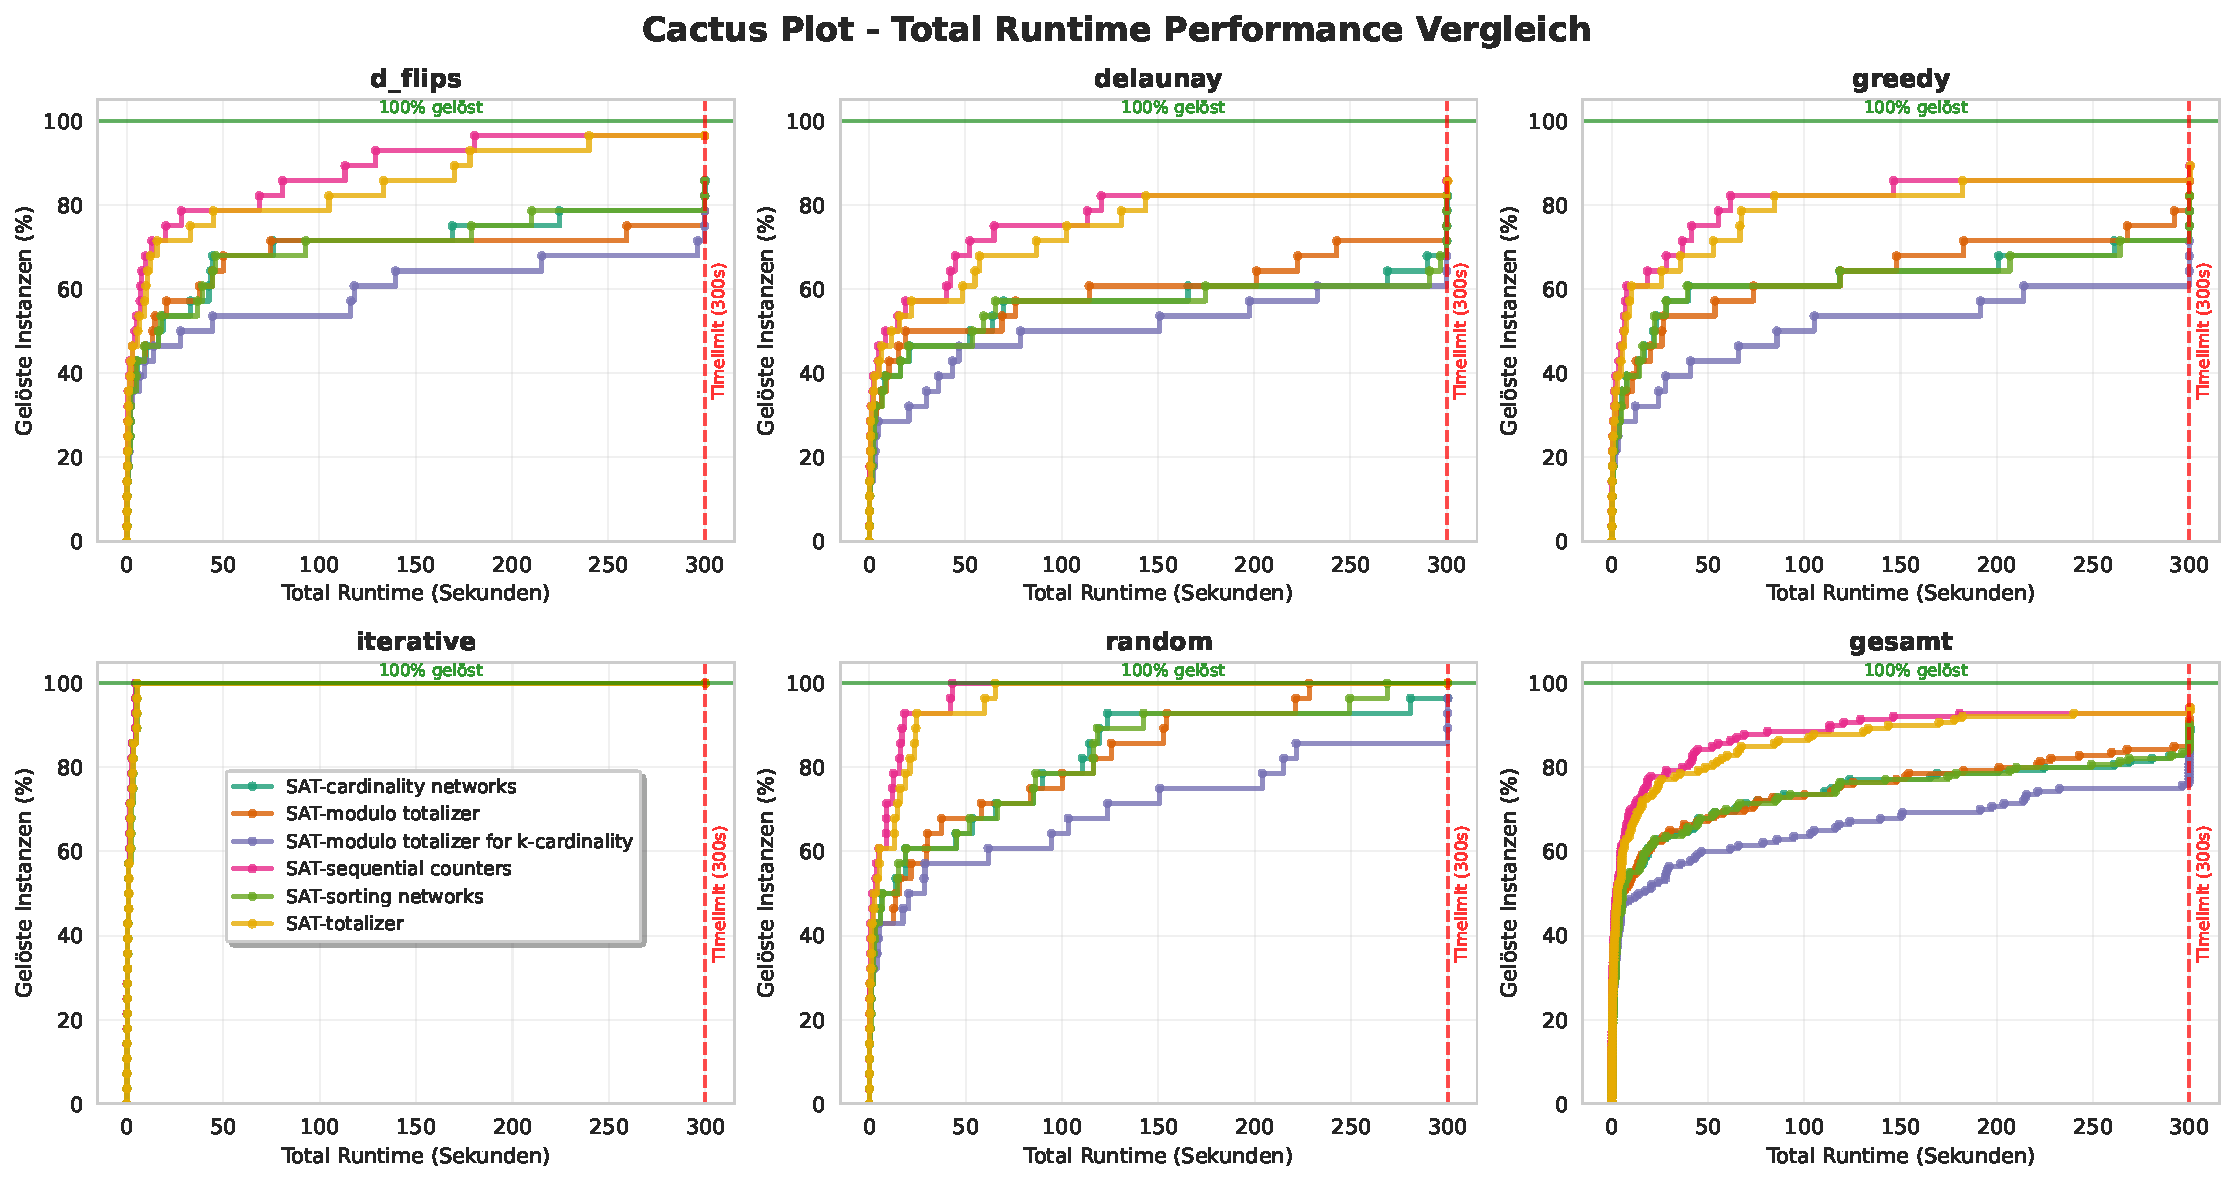
\includegraphics[width=1\linewidth]{eval5/exact.pdf}
    \caption{Die \emph{exact} Methode für die Gradbeschränkung  in einem SAT Solver, wurde mit verschiedenen Kardinalitätsbedingung getestet.}
    \label{fig:eval5_exact}
\end{figure}
\begin{figure}[htb]
    \centering
    
\includegraphics[width=1\linewidth]{eval5/atleast.pdf}
    \caption{Die \emph{atleast} Methode für die Gradbeschränkung  in einem SAT Solver, wurde mit verschiedenen Kardinalitätsbedingung getestet.}
    \label{fig:eval5_atleast}
\end{figure}


\end{document}
